% This is "sig-alternate.tex" V2.0 May 2012
% This file should be compiled with V2.5 of "sig-alternate.cls" May 2012
%
% This example file demonstrates the use of the 'sig-alternate.cls'
% V2.5 LaTeX2e document class file. It is for those submitting
% articles to ACM Conference Proceedings WHO DO NOT WISH TO
% STRICTLY ADHERE TO THE SIGS (PUBS-BOARD-ENDORSED) STYLE.
% The 'sig-alternate.cls' file will produce a similar-looking,
% albeit, 'tighter' paper resulting in, invariably, fewer pages.
%
% ----------------------------------------------------------------------------------------------------------------
% This .tex file (and associated .cls V2.5) produces:
%       1) The Permission Statement
%       2) The Conference (location) Info information
%       3) The Copyright Line with ACM data
%       4) NO page numbers
%
% as against the acm_proc_article-sp.cls file which
% DOES NOT produce 1) thru' 3) above.
%
% Using 'sig-alternate.cls' you have control, however, from within
% the source .tex file, over both the CopyrightYear
% (defaulted to 200X) and the ACM Copyright Data
% (defaulted to X-XXXXX-XX-X/XX/XX).
% e.g.
% \CopyrightYear{2007} will cause 2007 to appear in the copyright line.
% \crdata{0-12345-67-8/90/12} will cause 0-12345-67-8/90/12 to appear in the copyright line.
%
% ---------------------------------------------------------------------------------------------------------------
% This .tex source is an example which *does* use
% the .bib file (from which the .bbl file % is produced).
% REMEMBER HOWEVER: After having produced the .bbl file,
% and prior to final submission, you *NEED* to 'insert'
% your .bbl file into your source .tex file so as to provide
% ONE 'self-contained' source file.
%
% ================= IF YOU HAVE QUESTIONS =======================
% Questions regarding the SIGS styles, SIGS policies and
% procedures, Conferences etc. should be sent to
% Adrienne Griscti (griscti@acm.org)
%
% Technical questions _only_ to
% Gerald Murray (murray@hq.acm.org)
% ===============================================================
%
% For tracking purposes - this is V2.0 - May 2012

\documentclass{sig-alternate}
\usepackage[english]{babel}
\usepackage{blindtext}

\usepackage{etoolbox}
\makeatletter
\patchcmd{\maketitle}{\@copyrightspace}{}{}{}
\makeatother
\begin{document}
%
% --- Author Metadata here ---
%\conferenceinfo{WOODSTOCK}{'97 El Paso, Texas USA}
%\CopyrightYear{2007} % Allows default copyright year (20XX) to be over-ridden - IF NEED BE.
%\crdata{0-12345-67-8/90/01}  % Allows default copyright data (0-89791-88-6/97/05) to be over-ridden - IF NEED BE.
% --- End of Author Metadata ---

\title{Visible Light Position}
%
% You need the command \numberofauthors to handle the 'placement
% and alignment' of the authors beneath the title.
%
% For aesthetic reasons, we recommend 'three authors at a time'
% i.e. three 'name/affiliation blocks' be placed beneath the title.
%
% NOTE: You are NOT restricted in how many 'rows' of
% "name/affiliations" may appear. We just ask that you restrict
% the number of 'columns' to three.
%
% Because of the available 'opening page real-estate'
% we ask you to refrain from putting more than six authors
% (two rows with three columns) beneath the article title.
% More than six makes the first-page appear very cluttered indeed.
%
% Use the \alignauthor commands to handle the names
% and affiliations for an 'aesthetic maximum' of six authors.
% Add names, affiliations, addresses for
% the seventh etc. author(s) as the argument for the
% \additionalauthors command.
% These 'additional authors' will be output/set for you
% without further effort on your part as the last section in
% the body of your article BEFORE References or any Appendices.

\numberofauthors{5} %  in this sample file, there are a *total*
% of EIGHT authors. SIX appear on the 'first-page' (for formatting
% reasons) and the remaining two appear in the \additionalauthors section.
%
\author{
% You can go ahead and credit any number of authors here,
% e.g. one 'row of three' or two rows (consisting of one row of three
% and a second row of one, two or three).
%
% The command \alignauthor (no curly braces needed) should
% precede each author name, affiliation/snail-mail address and
% e-mail address. Additionally, tag each line of
% affiliation/address with \affaddr, and tag the
% e-mail address with \email.
%
% 1st. author
\alignauthor
Yen Su	\\
       \affaddr{National Taiwan University}\\
       \affaddr{Department of Electronic Engineering}\\
       \email{r03921080@ntu.edu.tw}
% 2nd. author
\alignauthor
Meng-Han Yang\\
       \affaddr{National Taiwan University}\\
       \affaddr{Department of Computer Sciencee and Information Engineering}\\
       \email{r03922120@ntu.edu.tw}
% 3rd. author
\alignauthor
Joe Haung\\
       \affaddr{National Taiwan University}\\
       \affaddr{Department of Computer Sciencee and Information Engineering}\\
       \email{r03922133@ntu.edu.tw}
\and  % use '\and' if you need 'another row' of author names
% 4th. author
\alignauthor
Wei-Chieh Kao\\
       \affaddr{National Taiwan University}\\
       \affaddr{Department of Computer Sciencee and Information Engineering}\\
       \email{r03922117@ntu.edu.tw}
\alignauthor
% 6th. author
\alignauthor
Wei-Cheng Lin\\
       \affaddr{National Taiwan University}\\
       \affaddr{Department of Computer Sciencee and Information Engineering}\\
       \email{r03922092@ntu.edu.tw}}
% There's nothing stopping you putting the seventh, eighth, etc.
% author on the opening page (as the 'third row') but we ask,
% for aesthetic reasons that you place these 'additional authors'
% in the \additional authors block, viz.
%\additionalauthors{Additional authors: John Smith (The Th{\o}rv{\"a}ld Group,
%email: {\texttt{jsmith@affiliation.org}}) and Julius P.~Kumquat
%(The Kumquat Consortium, email: {\texttt{jpkumquat@consortium.net}}).}
%\date{30 July 1999}
% Just remember to make sure that the TOTAL number of authors
% is the number that will appear on the first page PLUS the
% number that will appear in the \additionalauthors section.

\maketitle
\begin{abstract}
In this paper, we describe the design and implementation of Visible Light Positioning via camera on a smartphone as a receiver.With the pictures the camera received, we can use the position of the light in the pictures to estimate the smartphone's position. 
\end{abstract}

%\terms{Theory}

\keywords{Indoor localization; Mobile phones; Image processing}

\section{Introduction}
Positioning, also known as localization, is the process of determining the spatial position of an object or person. Accurate positioning is critical for numerous applications.{[2]} The implement of accurate indoor positioning enables a wide range of location-based services across many sectors. For example, shopping malls and supermarkets are suitable for indoor positioning because it can provide improved navigation which helps avoid unrealized sales when customers cannot find items they want, and it increases revenues from incremental sales from targeted advertising. However, the strong demand forecast, indoor positioning remains a "grand challenge", and no existing system offers accurate location and orientation using unmodified smartphones.\\
Accurate indoor positioning is not an easy task. Some challenges are still need to conquer. For example, the balance of cost of equipments and the accuracy of the measurement. The positioning error between the actual position and the computed result still has space to improve. How to real-timely compute the position while the smartphone is moving can also be a discussible issue.

\section{METHODLOGY}
The indoor positioning system consists of visible light beacons, mobile phones, and a cloudlet server.{[1]} Beacons transmit their identities or coordinates using visible light that human's eye is not perceptible. A smartphone receives these information by using its camera and then send the information to the cloud server to compute the position.
\begin{figure}[ht]
\begin{center}
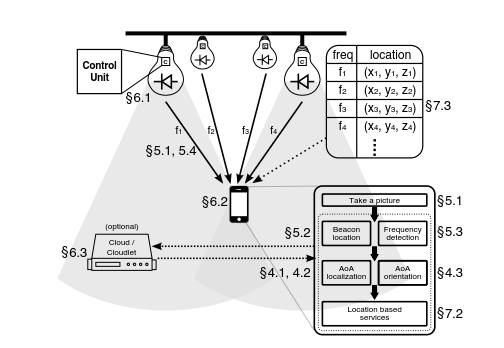
\includegraphics[scale=0.4]{1}
\caption{}
\end{center}
\end{figure}
\\
\subsection{Tools}
%Our design consists of visible light beacons, smartphones to determine a phone's location and orientation, and support location-based services.
Refer to the testbed in the paper, we consider using five LED beacons, smartphones, and a cloudlet server to compute.  
\section{Reference}
[1] Ye-Sheng Kuo, Pat Pannuto, Ko-Jen Hsiao, Prabal Dutta, Luxapose: Indoor Positioning with Mobile Phones and Visible Light Electrical Engineering and Computer Science Department, University of Michigan\\

[2] J.Armstrong, Y.A. Sekercioglu, and A. Neild. Visible light positioning: A roadmap for international %standardization.IEEE Communications Magazine, 51(12), 2013.
\end{document}  % This is where a 'short' article might terminate

%
% The following two commands are all you need in the
% initial runs of your .tex file to
% produce the bibliography for the citations in your paper.
%\bibliographystyle{abbrv}
%\bibliography{sigproc}  % sigproc.bib is the name of the Bibliography in this case
% You must have a proper ".bib" file
%  and remember to run:
% latex bibtex latex latex
% to resolve all references
%
% ACM needs 'a single self-contained file'!
%
%APPENDICES are optional
%\balancecolumns
